% Copyright 2026 Torbjörn E. M. Nordling
% SPDX-License-Identifier: Apache-2.0
% frame-step-02.tex — Step to 0.2: nothing happens (7:00–9:00)
% Article §3.1 and Fig. small: \SpeedAtTwo, \StartDuty, \SpeedAtStart, \StopDuty
% of data-article-results.tex (motor m5).
\begin{frame}{Step 1: duty 0.2 --- nothing happens}{P1 fails at the first experiment}
  \footnotesize
  \begin{columns}[T]
    \column{0.58\textwidth}
    \centering
    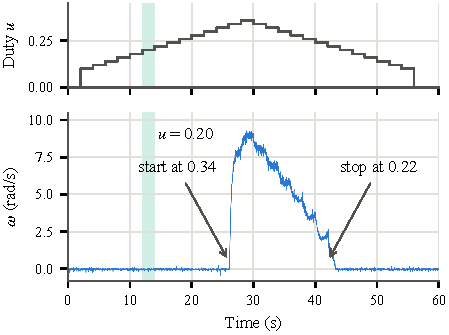
\includegraphics[width=\linewidth, height=0.8\textheight, keepaspectratio]{fig-small-duty.pdf}
    \column{0.4\textwidth}
    \scriptsize
    \begin{itemize}\setlength{\itemsep}{3pt}
      \item At duty 0.2: $\omega = \SpeedAtTwo$\,rad/s, \alert{at rest}.
      \item Raised, the wheel first turns at duty \StartDuty, at $\SpeedAtStart$\,rad/s.
      \item The linear model has no input below which the output stays zero.
      \item \textbf{Cause:} \alert{static friction} of motor and gears, which the torque must overcome before the rotor starts.
    \end{itemize}
    \alert{Not a fault:} check the wiring once, then record it as a result.
  \end{columns}
\end{frame}
